\documentclass{article}
\usepackage[english]{babel}
\usepackage{setspace}
\usepackage{graphicx}
\usepackage[colorlinks=true, allcolors=blue]{hyperref}
\usepackage[letterpaper,top=2cm,bottom=2cm,left=3cm,right=3cm,marginparwidth=1.75cm]{geometry}
\usepackage[utf8]{inputenc}
\setstretch{1.25}

\title{Investigation into the Methods of Choosing Presidential Electors and their Effects on Elections.}
\author{Caden Burkhardt and Eric D'Urso}
\date{May 2022}

\begin{document}

\maketitle

\begin{abstract}
    In order to become president, a candidate must win 270 electoral votes from the 50 states and DC; however, because of Federalism and the Tenth Amendment’s reserved powers for states, how each state chooses to select their electors varies from state to state. This study used election data from the three most recent US presidential elections to test how various permutations in how states choose their electors affect the outcome of the general election and analyzed the data generated.
\end{abstract}

\section{Introduction}
The United States presidential election is arguably the most important election in the United States. Who the voting public chooses will represent the nation for the following four year, and will wield significant power.  Recently, there has been much scrutiny over the process we use to choose our president. Not only has there been controversy over the 2020 presidential election, but controversy has been present in the 2016, 2004, 2000, elections. Going further back there have been controversies in 1888, 1876, and 1824. Much of this controversy can be traced back to the electoral college, the procedures established in the US Constitution to choose the US president. 

According to the electoral college, each state receives a number of electors, equal to the number of US Representatives and Senators the state has combined, or three for the District of Columbia. The electors then meet and vote for president, with a majority of the 270 electoral votes required to carry the election. In this procedure, how electors are chosen is determined by the individual states. As such, different states use different methods to determine their electors. Most states utilize a winner-take-all system, where the political party that wins the majority of popular votes in the state, gets to choose all of the state's electors. However, Maine and Nebraska utilize a congressional district system, where the state allocates electors to the winners of the states’ congressional districts as opposed to the winner of the popular election. The congressional district system splits the electoral votes, diluting the amount of electoral votes won when a party wins the popular vote in a state.

Our goal with this paper is to utilize our understanding of the various ways electors are chosen and apply them, using a simulation to test how various permutations in how states choose their electors affect the outcome of the general election. For example, Texas is traditionally a very red state, voting for republican candidates since 1980 and awarding all 38 electoral votes to them. However, the state still has 13 blue congressional districts. If Texas were to change the method of choosing electors from a winner take all system to a congressional district system, the democratic party would gain about 13 electoral votes from Texas that they would not have received under the winner take all system.  Our simulation runs the numbers to calculate the outcome of changing various states from a winner-take-all method, to a congressional district method, and measuring the effect on the outcome of the elections. We are looking to find results that would have changed the 2012, 2016, or 2020 election results, and analyze that data.

\section{Methods}
We decided to specifically take data from the three most recent presidential elections, 2012, 2016 and 2020. For our simulations we used two different data sets. One showed the voter results for the presidential election in each state’s congressional districts \cite{kos}, and the other showed the popular vote results from each state \cite{pop}. These datasets, however, were not complete in that they did not include any data from the District of Columbia, so this data was obtained separately for 2012 \cite{dc3}, 2016 \cite{dc2}, and 2020 \cite{dc1}. The first step in running our simulation is preprocessing the data. We put both data sets into a script which combines and simplifies each state into four data points: state name, Winner in a winner-take-all system, number of votes won by each party (republican and democrat) in a congressional district method system.

Once we have our newly generated dataset, we run that through a new script which uses a brute force computing approach to simulate various election possibilities. The script initially tested every possible combination of congressional district voting and winner-take-all voting for all 50 states and DC, resulting in 2\textsuperscript{51} possible combinations. Unfortunately, we did not have the computing power to run that many calculations, so we had to streamline our code by eliminating combinations where we change the election’s losers states from winner-take-all  to congressional district method as that would only split the losing parties vote and widen the winners voting margin, as well as all scenarios where all of a states congressional districts were carried by the winner of the popular vote, since how electoral votes are distributed does not change between the two methods. By eliminating states that fall under this criteria, we only test our simulation on states that could have contributed to changing the outcome of the election if they were flipped. This left us with exactly 18 states for each of the simulations to run (on the years 2012, 2016, and 2020) and only 2\textsuperscript{18} combinations to compute, making the streamlined process significantly more efficient. Still with that many combinations, each simulation took over five hours.

The scripts and datasets mentioned above can now be found \href{https://github.com/edurso/gov-action-project}{here on GitHub}.

\section{Results}
Once all of the simulations were complete we received an output showing all simulated combinations where the outcome of the election was altered and a list of the states whose method of selecting electors was altered to achieve this new outcome.

For the 2012 election (\hyperref[fig:2012]{Figure 1}), 72.6\% of the simulated outcomes still predicted the democratic candidate, Barack Obama to win, with 25.4\% of the simulated outcomes flipping the results and challenger Mitt Romney winning, and 2.0\% of outcomes where there is a perfect electoral split, in which case the House of Representatives would decide the winner.

\begin{figure}
\centering
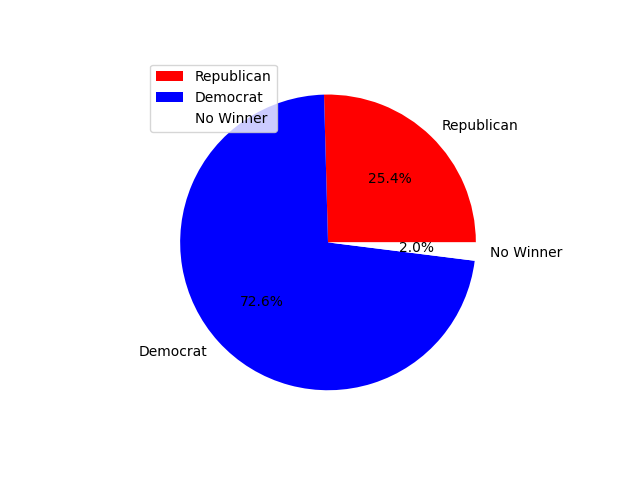
\includegraphics[width=0.85\textwidth]{data-2012.png}
\caption{\label{fig:2012}Results of 2012 Simulation}
\end{figure}

For the 2016 election (\hyperref[fig:2016]{Figure 2}), the results were much closer with only 50.0\% of the simulated outcomes still predicted for the republican candidate, Donald Trump to win, with 46.8\% of the simulated outcomes flipping the results predicting that Hillary Clinton would have won, and 3.2\% of outcomes where there is a tie

\begin{figure}
\centering
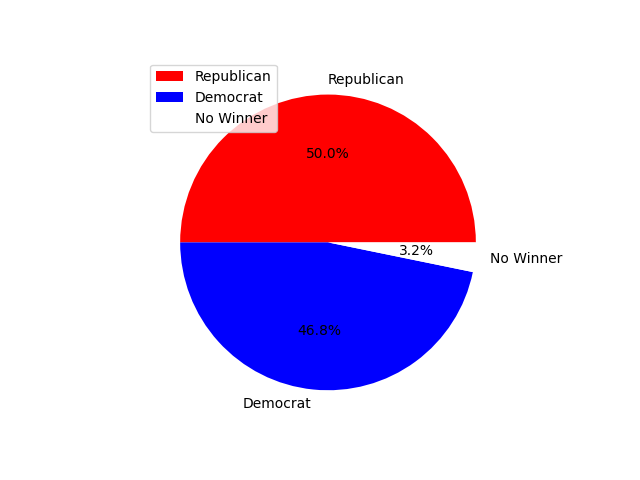
\includegraphics[width=0.85\textwidth]{data-2016.png}
\caption{\label{fig:2016}Results of 2016 Simulation}
\end{figure}

For the 2020 election (\hyperref[fig:2020]{Figure 3}), a majority of simulations, 67.0\%, predicted that Donald Trump would have won re-election with only 30.1\% of simulations having the democratic candidate Joe Biden winning and 2.9\% of simulated elections ending with a tie.

\begin{figure}
\centering
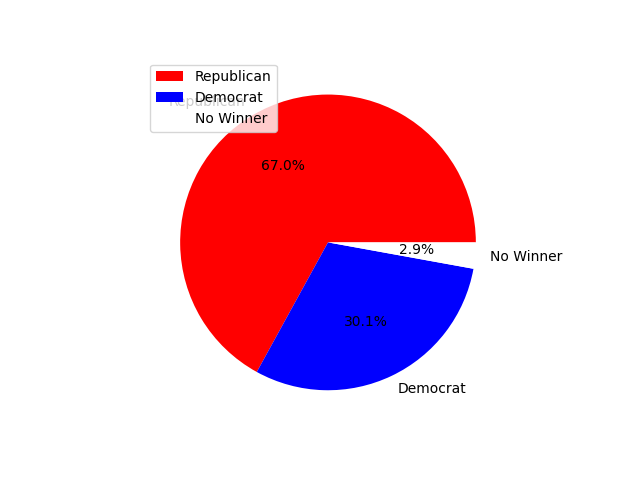
\includegraphics[width=0.85\textwidth]{data-2020.png}
\caption{\label{fig:2020}Results of 2020 Simulation}
\end{figure}

In addition, we calculated the percent of scenarios that each state showed up in with the states with a greater effect on the outcome of an election showing up more frequently. This is depicted in \hyperref[fig:t2012]{Figure 4}, \hyperref[fig:t2016]{Figure 5}, and \hyperref[fig:t2020]{Figure 6}.

\begin{figure}
\centering
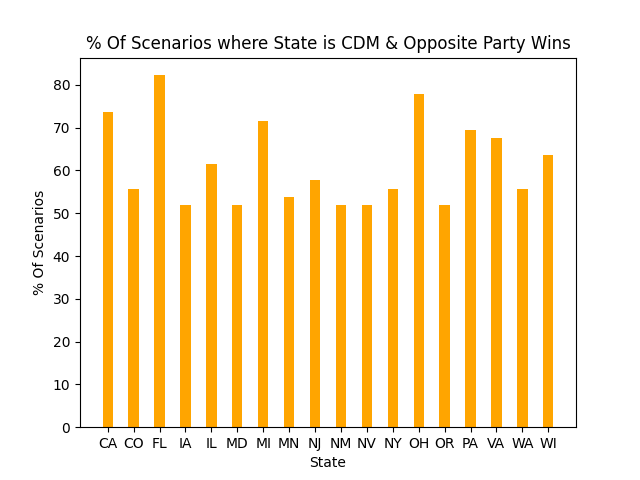
\includegraphics[width=0.75\textwidth]{trend-2012.png}
\caption{\label{fig:t2012}Trends of 2012 Simulation}
\end{figure}

\begin{figure}
\centering
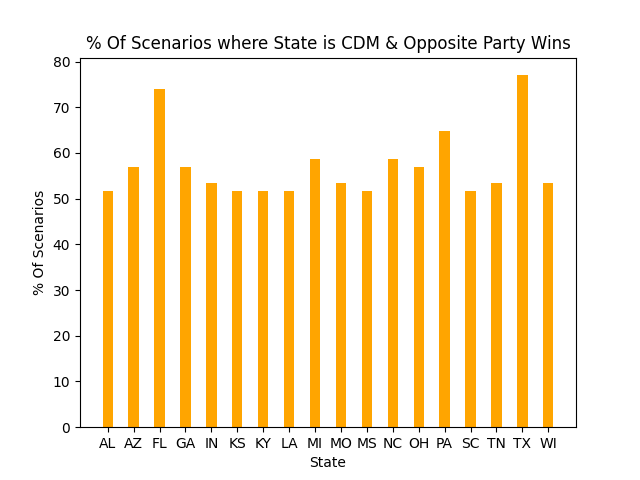
\includegraphics[width=0.75\textwidth]{trend-2016.png}
\caption{\label{fig:t2016}Trends of 2016 Simulation}
\end{figure}

\begin{figure}
\centering
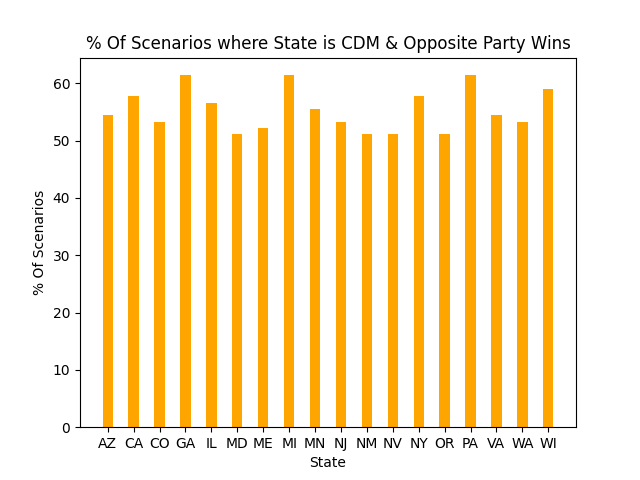
\includegraphics[width=0.75\textwidth]{trend-2020.png}
\caption{\label{fig:t2020}Trends of 2020 Simulation}
\end{figure}

\section{Discussion}
We can draw a couple of interesting conclusions from the data we have collected. Firstly, it is possible, without changing how people vote, to change the outcome of an election based on states deciding to choose their electors. However, no single state could have influenced the outcome of the election itself; all combinations where an election result was flipped required more than one state. Even though no single state could have changed the outcome of the election, certain states have more of an impact than others. Larger states, such as California, Texas and Florida as well as battleground states such as Ohio, Michigan and Pennsylvania were in a greater percent of outcomes where the simulated election results were flipped. We believe this to be because these states tend to have a numerically larger number of minority controlled districts so by changing to the congressional district method a larger number of electoral votes are won.

While it is probably very unlikely that large states such as California, Texas and Florida would want to change how they choose their electors, since the controlling party would simply be giving electoral votes to their political rivals, it may be worth considering for swing states. For example, Michigan tends to vote Democratic for most national elections, but at the state level, republicans control the state legislature. If it may be beneficial for them to change their process for choosing electors would split the number of electoral votes the Democratic Party would get and increase the number of electoral votes the republicans would get. However, this would be risky as if a Republican candidate, like Donald Trump in 2016, is able to swing Michigan red, then Michigan using the congressional district method would award electors to the democratic party that would have gone to the republican party under a winner-take-all system.

In addition, This project has shown us just how increasingly volatile the electoral college system is becoming. In 2012 the winning party(D) still won a majority (72.6\%) of simulated elections. In the simulated 2016 elections, the winning party(R) won a plurality (50.0\%). Surprisingly, for 2020, the winning party(D) only won 30.1\% of simulated elections. This is in stark contrast to the 2012 election where the winning party which also happened to be democratic over double of the simulated elections. Because all of the simulated elections had at least one state change how it chooses its electors, this shows changing how a state chooses its electors is having a greater impact on elections now than ever.

\section{Conclusion}
In our project we have explored the ways in which a state chooses its electors can affect the outcome of the US general election. We believed that by changing the methods states use to choose their electors, we could affect the outcome of our simulated elections. Indeed, we found numerous combinations of states that could have flipped the 2012, 2016, and 2020 election results. Specifically, we found that larger states and swing states had a larger impact on changing an election than others. Moreover, we concluded that elections are becoming more volatile, as more simulated elections, and therefore more different combinations of  methods of choosing electors lead to flipped election results as time has gone on. The electoral college is not perfect. We have simply found and explored one way to exploit the system.

\bibliographystyle{ieeetr}
\bibliography{cite}

\end{document}
